% !TEX root = main.tex

\vphantom{}\marginnote{
    
\includegraphics[width=0.8\linewidth]{assets/techjam-2018.eps}
    
    \bigskip
    
\includegraphics[width=0.8\linewidth]{assets/code-squad.eps}
}%
{\techjam}\;\; เป็นการแข่งขันที่จัดขึ้นโดย {\ltspc KBTG} เพื่อเฟ้นหาสุดยอดขุนพลแห่งอนาคตด้าน
\textit{Coding},\, \textit{Data Science} และ\, \textit{Design} 
ที่ผู้เข้าร่วมแข่งขันเปรียบเสมือนขุนพลจากทั่วประเทศที่จะนำทักษะความสามารถทางเทคโนโลยีและการออกแบบ
ซึ่งเป็นเครื่องมือสำคัญของยุคสมัยแห่งอนาคต มาประชันกันเพื่อหาสุดยอดฝีมือ

ในการแข่งขันของกลุ่ม Code Squad นั้นเราต้องการค้นหาสุดยอดฝีมือด้านการเขียนโปรแกรมและพัฒนาซอฟต์แวร์ที่มีความสามารถรอบด้าน\;
เราเชื่อว่านักพัฒนาซอฟต์แวร์ที่ดี นอกจากจำเป็นจะต้องมีทักษะการเขียนโปรแกรมที่เก่งกาจแล้ว
ยังต้องมีความสามารถที่จะเข้าใจและวิเคราะห์ปัญหาในเชิงนามธรรมและระดับโครงสร้างได้
และยังต้องสามารถเลือกใช้วิธีแก้ปัญหาที่เหมาะสมกับเงื่อนไขและตัวแปรข้อจำกัดต่าง ๆ ได้ดีอีกด้วย

ในการแข่งขัน Code Squad นั้น เราจึงออกแบบโจทย์ให้มีความหลากหลาย ท้าทาย และอาจไม่เคยพบเห็นที่ใดมาก่อน\;
โจทย์แต่ละข้อจะวัดทักษะการเขียนโปรแกรมหรือความรู้ที่เกี่ยวกับการแก้ปัญหาเชิงคำนวณด้วยคอมพิวเตอร์
ตลอดจนไปถึงการนำทักษะและความรู้ดังกล่าวมาแก้ปัญหาที่สลับซับซ้อนมากขึ้น\;
ในขณะเดียวกันนี้เราพยายามปรับสมดุลโจทย์ให้เข้าใจได้ไม่ยาก แต่ยังคงไว้ซึ่งความเข้มข้นของการไขโจทย์ไว้อย่างครบเครื่อง

ทีมงานได้คัดเลือกโจทย์ที่ใช้แข่งขันของกลุ่ม Code Squad จากงาน {\techjam} นำมารวบรวมและเรียบเรียงไว้ในเอกสารฉบับนี้ 
เพื่อเป็นประโยชน์แก่นักเรียน นักศึกษา และบุคคลทั่วไปที่สนใจเรื่องการพัฒนาซอฟต์แวร์และการศึกษาที่เกี่ยวกับวิทยาการคำนวณและวิทยาการคอมพิวเตอร์ 
อันเป็นแรงบันดาลใจให้นักเรียน นักศึกษา นักเขียนโปรแกรมและผู้ที่สนใจในเทคโนโลยีได้ศึกษาค้นคว้าความรู้ต่อไป

หวังว่าผู้อ่านจะสนุกและเรียนรู้ไปพร้อมกับการแก้ปัญหาโจทย์ปัญหาที่ท้าทายเหล่านี้

\begin{flushright}
\twoemrule\ ทีมงาน Code Squad, {\techjam}
\end{flushright}


\newpage\noindent
{\sectionfont \llap{$\blacklozenge$\; }โจทย์ที่ใช้แข่งขันมีลักษณะอย่างไร?}

\smallskip\noindent
โจทย์ที่ใช้แข่งขันในกลุ่ม Code Squad นั้นแบ่งออกได้เป็นสามประเภทใหญ่ ๆ คือ

% TODO: instead of enumeration, use logo from fontawesome
\begin{enumerate}
    \item \textbf{Quickfire}\; 
        เป็นโจทย์ที่ต้องใช้ไหวพริบแล้วความรวดเร็วในการตอบคำถาม ภายในเวลา 10{\hrsp--\hrsp}60 วินาที\;
        ผู้เข้าแข่งขัน\textit{ไม่}สามารถใช้คอมพิวเตอร์เพื่อช่วยแก้ปัญหาเหล่านี้ได้ 
    \item \textbf{Ponder}\;
        เป็นโจทย์ที่ต้องใช้เวลาในการพิจารณาคำถามและค้นหาคำตอบภายใน 5 นาที\;
        ผู้แข่งแข่งขันสามารถใช้คอมพิวเตอร์หรือเทคนิคใด ๆ ก็ได้เพื่อช่วยแก้ปัญหาเหล่านี้ได้\;
        หากผู้เข้าแข่งขันสามารถค้นหาคำตอบได้ถูกต้องและรวดเร็วกว่าคนอื่น ๆ ก็จะได้คะแนนสูงขึ้นตามไปด้วย
    \item \textbf{Coding}\;
        เป็นโจทย์ปัญหาเชิงอัลกอริทึมที่ผู้เข้าแข่งขันต้องเขียนโปรแกรมเพื่อช่วยค้นหาคำตอบอย่างมีประสิทธิภาพ
        ตามสเปกที่กำหนด
\end{enumerate}

\medskip\noindent
{\sectionfont \llap{$\blacklozenge$\; }โจทย์เหล่านี้มีเฉลยหรือไม่?}

\smallskip\noindent
ถึงแม้ว่าโจทย์เหล่านี้จะมีคำตอบที่ถูกต้องชัดเจนอยู่แล้วทุกข้อ (เว้นคำถามข้อสุดท้าย)
แต่ในขณะนี้ทางทีมงานยังไม่มีแผนที่จะจัดและเผยแพร่เฉลยของโจทย์เหล่านี้อย่างเป็นทางการ

อย่างไรก็ดีทางทีมงานมีความยินดีเป็นอย่างยิ่ง หากผู้อ่านท่านใดเลือกที่จะนำเสนอวิธีที่ใช้ไขปัญหาโจทย์ข้อต่าง ๆ
ในรูปแบบของบทความหรือสื่ออื่นใด อันจะเป็นประโยชน์แก่สาธารณะได้


\vspace*{\fill}

\begin{small}
    \bigskip\noindent
    {\textcopyright} สงวนลิขสิทธิ์ 2561{\hrsp--\hrsp}2562\; กสิกร บิซิเนส{\hrsp--\hrsp}เทคโนโลยี กรุ๊ป \\
    ตามพระราชบัญญัติลิขสิทธิ์ พุทธศักราช 2537

    \smallskip\noindent
    เอกสารฉบับนี้ถูกเผยแพร่ภายใต้สัญญาอนุญาต Creative Commons Attribution--NonCommercial 4.0 International
    ซึ่งอนุญาตให้ทำซ้ำ แจกจ่าย หรือแสดงและนำเสนอเอกสารฉบับนี้ และสร้างงานดัดแปลงจากเอกสารฉบับนี้\;
    โดยต้องให้เครดิตและแสดงที่มาและไม่ใช้เพื่อการค้า

    \smallskip\noindent
    อ่านเงื่อนไขฉบับเต็มได้ที่\; \url{https://creativecommons.org/licenses/by-nc/4.0/} 

    \bigskip\noindent
    \includegraphics[width=0.190983\linewidth]{assets/by-nc.eps}

    \medskip\noindent
    พัฒนาโดยใช้ {\XeLaTeX} เมื่อ \texttt{\DTMtoday} เวลา \texttt{\DTMcurrenttime}

    \smallskip\noindent
    ติดต่อสอบถามหรือติดตามรายละเอียดเพิ่มเติมได้ที่\; \url{https://techjam.tech}
    
\end{small}
